\subsection{Consolidamento Requisiti}

\textbf{Periodo:} dal 2020-01-14 al 2020-01-18
\\La fase inizia appena terminata la precedente e finisce con la presentazione della \textit{Revisione dei Requisiti}.
\\Le precondizioni sono:
\begin{itemize}
    \item Le postcondizioni della fase precedente sono state soddisfatte;
    \item Consegna dei documenti richiesti al proponente.
\end{itemize}
Le postcondizioni sono:
\begin{itemize}
    \item Ultimata preparazione della presentazione da esporre in sede di revisione;
    \item Ogni componente ha studiato le tecnologie necessarie;
\end{itemize}


\subsubsection{Diagramma di Gantt: Consolidamento Requisiti}
\begin{figure}[ht]
    \centering
    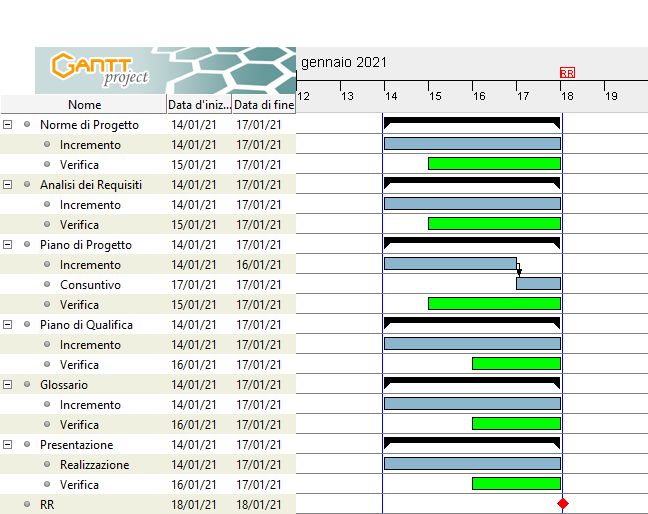
\includegraphics[width=\textwidth]{../../Immagini/Consolidamento.png}
    \caption{Diagramma di Gantt dell'avvitià di Consolidamento dei Requisiti}
\end{figure}
